\section{Task 1: Reading and Writing Grayscale Images}

The first step in this lab is to load an image using imread. When Matlab loads
an image , it takes th image file, whatever format it is saved in, and stores
the raw image data in a two-dimension array. We want to end the line containing
the call to imread with a semicolon so that it does not print the value of every
pixel to the console. We also can extract additional information on our first
image, barbara.jpg, using functions iminfo, whos, and size. The
console output is shown below:

\begin{itemize}

    \item \textbf{iminfo:}
    
    \lstinputlisting{iminfoDump.txt}

    \item \textbf{whos:}

    \lstinputlisting{whosDump.txt}

    \item \textbf{size:}

    \lstinputlisting{sizeDump.txt}

\end{itemize}

So here we can see that barbara is a 256x256 image made up of uint8 (unsigned
8-bit integers).

In order to view barbara we use imshow. Providing only the image object as an
argument simply displays the image, but if we also provide a 1x2 matrix [a, b]
the function will make all pixels with an intensity less than a black and all
pixels above b to be white. Providing an empty matrix performs auto contrast
adjustment, transforming intensity values to maximize contrast without losing
information.

\begin{figure}[H]
    \centering
    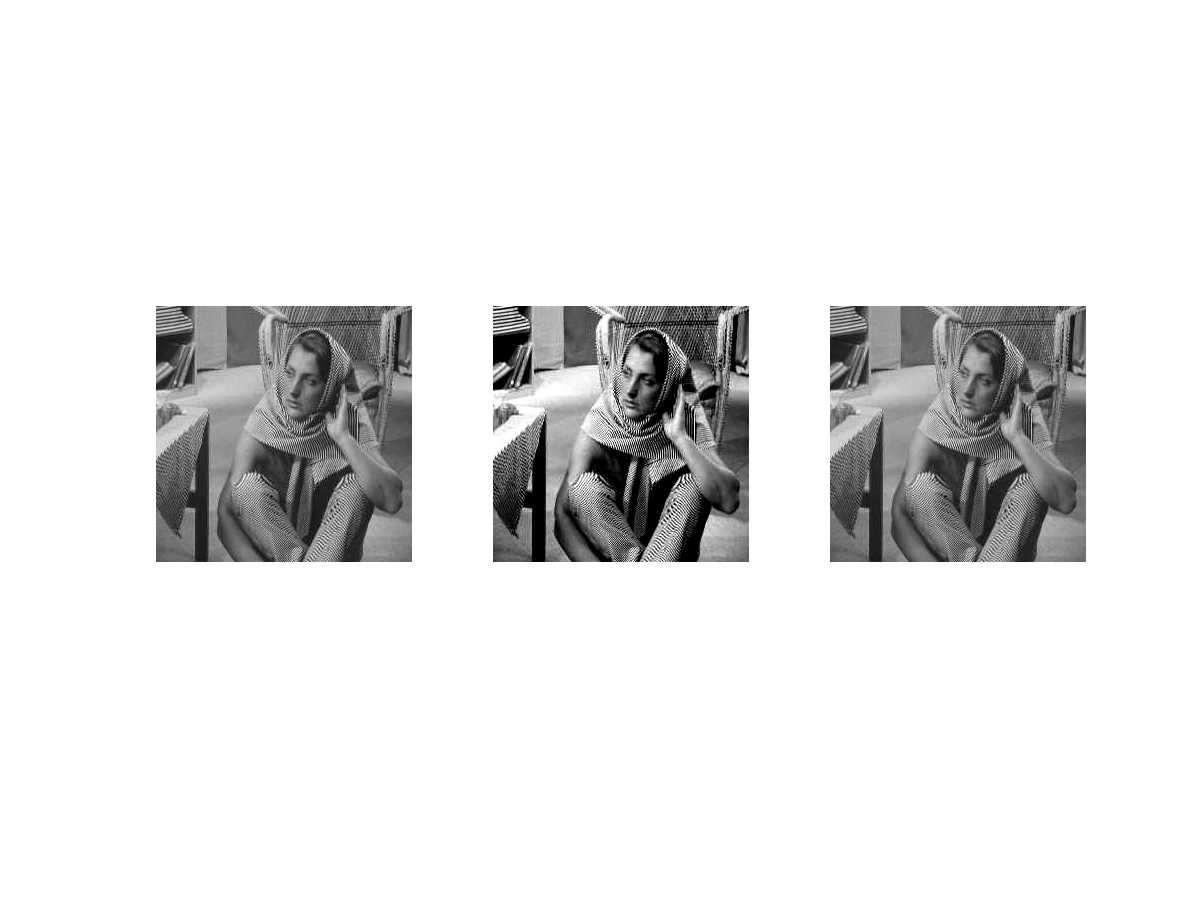
\includegraphics[scale=0.5]{imshow}
    \caption{Output of imshow providing nothing, [a, b], and [] for the second
    argmument}
\end{figure}

The imtool function can be used to zoom into the chosen image, view pixel
intensity values, and alter them. I used this function to explore some of the
values in barbara, alter them, and see the affect of those changes zoomed out.

In Matlab we can save image objects to a file using imwrite and we can save them
under different quality levels. In this example we save lena.tiff and see the
effects of saving it at different quality levels:

\begin{figure}[H]
    \centering
    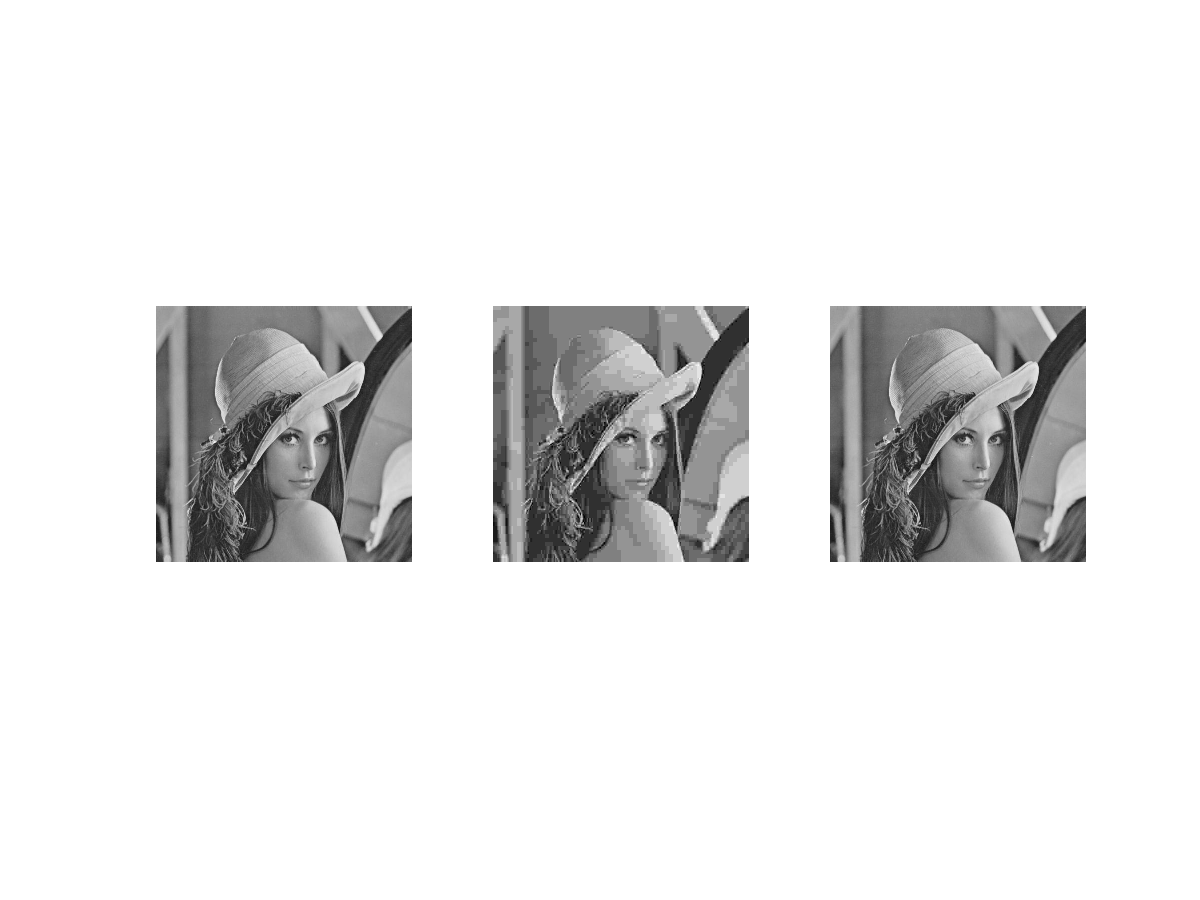
\includegraphics[scale=0.5]{lenaCompare}
    \caption{Comparison of lena saved at different qualities}
\end{figure}

The images are saved at smaller sizes when quality is decreased. For example,
lena3 is 32x32. Matlab seems to view lena3 at the same size as the other two
images, and hence applied a scaling transformation to do so (probably using
linear interpolation). This is why we are not viewing it as large pixels, but a
very blurry image.
